\section{The \pktlanguage compiler backend}
\subsection{Expression flattening to three-address code}
As a first step, we convert code into three-address code, where all
instructions are either reads / writes into stateful variables or carry out
packet manipulations of the form: \texttt{pkt.f1 = pkt.f2 op pkt.f3;} where
\texttt{op} includes all arithmetic, logical, and relational operators. We also
allow either pkt.f2 or pkt.f3 to be an opaque function call of multiple packet
fields, because \pktlanguage assumes opaque functions are supported in
hardware. Three-address code instructions are similar to P4's action primitives
~\cite{p4spec} and map one-to-one with RMT~\cite{rmt}'s VLIW instruction set.

To generate three-address code, we flatten expressions that are not
already legal three-address code, by introducing enough temporaries. For
instance, \texttt{pkt.f = pkt.f1 + pkt.f2 - pkt.f3;} would be flattened to
\texttt{pkt.tmp = pkt.f2 - pkt.f3;} followed by \texttt{pkt.f = pkt.f1 +
pkt.tmp;}

\begin{figure}[!h]
\begin{tiny}
\begin{lstlisting}
pkt.id00 = hash2(pkt.sport, pkt.dport) % 8000;
pkt.saved_hop00 = saved_hop[pkt.id00];
pkt.id10 = hash2(pkt.sport, pkt.dport) % 8000;
pkt.last_time00 = last_time[pkt.id10];
pkt.new_hop0 = hash3(pkt.sport, pkt.dport, pkt.arrival_time) % 64;
pkt.tmp1 = pkt.arrival_time - pkt.last_time00;
pkt.tmp00 = pkt.tmp1 > 5;
pkt.saved_hop01 = (pkt.tmp00) ? (pkt.new_hop0) : pkt.saved_hop00;
pkt.last_time01 = pkt.arrival_time;
pkt.next_hop0 = (pkt.tmp00) ? (pkt.new_hop0) : pkt.saved_hop00;
saved_hop[pkt.id00] = (pkt.tmp00) ? (pkt.new_hop0) : pkt.saved_hop00;
last_time[pkt.id10] = pkt.arrival_time;
\end{lstlisting}
\end{tiny}
\caption{Flowlet switching in three-address code}
\label{fig:three_address}
\end{figure}

\subsection{Code partitioning}
At this point, the code is still in sequential form. Code partitioning
turns sequential code into an atom grid that can be run by \absmachine , by
exploiting parallelism within and across pipeline stages.
To partition code, we carry out the following steps:
\begin{enumerate}
  \item Create a node for each statement in the packet transaction after
    expression flattening.
  \item Create a bidrectional edge between N1 and N2 where N1 is a read from a
    state scalar / state array and N2 is a write into the same state scalar /
    state array. This step captures the constraint that state is internal to an
    atom in \absmachine.
  \item Create an edge (N1, N2) for every pair of nodes N1, N2 where N2 reads
    a variable written by N1. This is the only dependency we need to check because
    control dependencies turn into data dependencies when generating straight-line
    code. Further, the use of SSA removes all write-after-read and write-after-write
    dependencies.
  \item Generate strongly connected components (SCCs) of the resulting graph
    (Figure~\ref{fig:deps}) and condense the SCCs to to create a directed
    acyclic graph (DAG) (Figure~\ref{fig:dag}). This step captures the
    constraint that all updates to state variables must reside within the same
    atom.
  \item Schedule the resulting DAG using critical path
    scheduling~\cite{crit_path_sched}, creating a new pipeline stage everytime
    one operation needs to follow another (Figure~\ref{fig:pipeline}).
\end{enumerate}

\begin{figure*}
  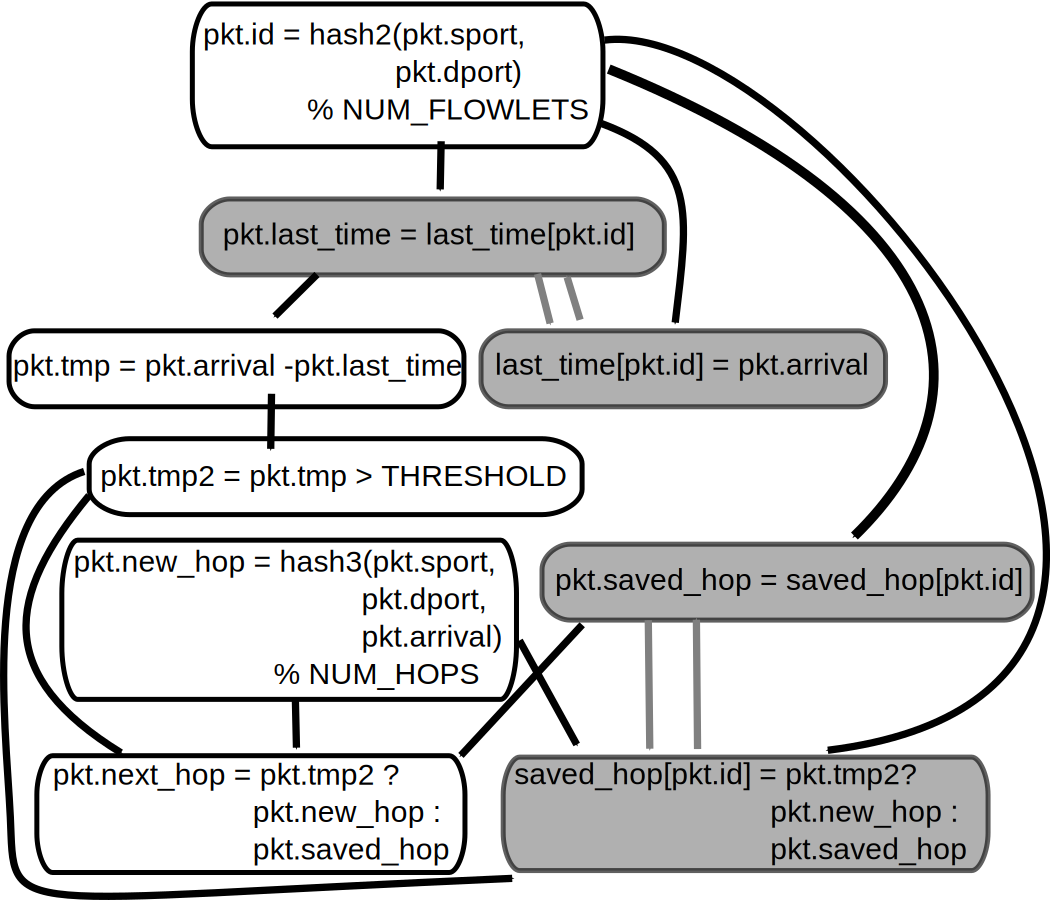
\includegraphics[width=\textwidth]{deps.pdf}
  \caption{Dependency graph of code shown in Figure~\ref{fig:three_address}}
  \label{fig:deps}
\end{figure*}

At this point, each strongly connected component can be turned into an atom for
\absmachine and the resulting pipeline implements the packet transaction.
Further, the atoms have a very stylized form. Stateless atoms contain exactly
one three-operand code instruction. Atoms that manipulate state contain at
least two statements: a read from a state variable and a write to a state
variable and optionally consist of one or more updates to the state variable.

\subsection{Respecting constraints on atoms}

So far, we haven't constrained the code in atom bodies in any way to reflect
hardware constraints. Expression flattening generates stateless atoms that each
have only one instruction. Further, because these instructions are in
three-operand code form, they map directly to the VLIW capabilities of
programmable switches.

Atoms that manipulate state can, in general, have multi-line atom bodies and it
is unclear whether these can be implemented at all. For instance, the update to
the state variable \texttt{saved\_hop} requires a read, followed by a
conditional update, followed by a write back. This section develops a general
technique to determine the implementability of stateful atoms, given
constraints on stateful atom bodies imposed by the hardware.

We first observe that constraints on stateful atoms can be written as program
sketches~\cite{bitstreaming, finite, sketch_manual}: a code fragment with fixed
and configurable parts. For instance, an atom with the constraint that it can
execute at most one programmable modify operation between a read and a write
operation to a stateful variable x can be represented as:
\begin{figure}
\begin{tiny}
\begin{lstlisting}
pkt.tmp = x;
pkt.tmp2 = pkt.tmp ?? (??);
x = pkt.tmp;
\end{lstlisting}
\end{tiny}
\caption{Sketch for single update operation to a state variable}
\label{fig:sketch_for_state}
\end{figure}
Here, the double question mark \texttt{??} stands for a
\textit{hole}~\cite{sketch_manual}. The hole is a placeholder for values from a
finite set that can be substituted in place of the hole. An automated program
synthesis~\cite{synthesis} tool called Sketch~\cite{sketch_manual} then
\textit{fills in} these holes to make the sketch equal to a specification.

As an example, if we want to implement the specification \texttt{x = x + 1;}
using the sketch in Figure~\ref{fig:sketch_for_state}, the Sketch tool would
fill the first hole with the value '+' from the finite set ('+', '-', '/', '*')
and the second hole with the value 1 from a finite set of integers specified as
input to the tool.

For the interested reader, a more detailed explanation of how Sketch works is
available in the appendix. For the purposes of the \pktlanguage compiler
though, we treat Sketch as a blackbox. We express the underlying constraints on
atoms as sketches, feed Sketch with an atom specification that needs to be
satisfied.  If there is a way to complete the sketch to satisfy the atom
specification, Sketch will find it, otherwise, it will determine that the
specification is unsatisfiable. For instance, the specification: \texttt{x = x
* x;} is unsatisfiable given the constraints in
Figure~\ref{fig:sketch_for_state}.

Using sketches to model constraints on atoms allows us to express constraints
very generically. At its core, a sketch is an incomplete imperative program,
and hence can express a variety of atom constaints. To show its generality, we
conside two such constraints in our evaluations: an in-order sequential CPU
that can execute exactly $N$ three-operand instructions and a combinatorial
circuit with a very specific form.

\begin{figure}
  \includegraphics[width=\columnwidth]{dag.pdf}
  \caption{DAG formed by condensing SCCs in Figure~\ref{fig:deps}}
  \label{fig:dag}
\end{figure}
